\documentclass{beamer}

\mode<presentation>
{
  \usetheme{% Tema de la presentaci'on (colores, formas, etc.)
    AnnArbor%
    %Antibes%
    %Bergen%
    %Berkeley%
    %Berlin%
    %Boadilla%
    %boxes%
    %CambridgeUS%
    %Copenhagen%
    %Darmstadt%
    %default%
    %Dresden%
    %Frankfurt%
    %Goettingen%
    %Hannover%
    %Ilmenau%
    %JuanLesPins%
    %Luebeck%
    %Madrid%
    %Malmoe%
    %Marburg%
    %Montpellier%
    %PaloAlto%
    %Pittsburgh%
    %Rochester%
    %Singapore%
    %Szeged%
    %Warsaw%
  }

  \setbeamercovered{transparent} % Opcional para la aparicion gradual
}


\usepackage[english]{babel} 

\title{Proyecto}

\subtitle{Factorizaci\'on de enteros}

\author[Mart\'inez] 
{Gabriel Mart\'{i}nez Gonz\'alez}

\institute[ESFM] 
{
  Escuela Superior de F\'{\i}sica y Matem\'aticas\\
  Instituto Polit\'ecnico Nacional}

\date[\today]{\today}


%\beamerdefaultoverlayspecification{<+->} % Por si se quiere que aparezca
                                          % gradualmente los items


\begin{document}

\begin{frame}
  \titlepage
\end{frame}

\begin{frame}
  \frametitle{Divisi\'on por tentativa}

  \tableofcontents
\end{frame}

\section{Teor\'{i}a detr\'as del algoritmo}

\begin{frame}
  \frametitle{Ideas principales}
  \framesubtitle{Analis\'{i}s del n\'umero 2 como factor}

  \begin{itemize}[<+->] % para que parezcan uno a uno
  \item Consideremos $n$ un n\'umero entero positivo.
  \item Si $n(mod2)=0$, 2 es factor de $n$ y $\frac{n}{2}$ es el factor m\'as grande que podr\'{i}amos tener.
  \item $\frac{n}{2}$ no tiene por qu\'e ser primo.
  \item S\'olo basta comprobar los n\'umeros $q$, tales que $q\leq\frac{n}{2}$
  \end{itemize}
\end{frame}
\begin{frame}
  \frametitle{Ideas principales}
  \framesubtitle{Extensi\'on a otro primos}

  \begin{itemize}[<+->] % para que parezcan uno a uno
  \item Se puede aplicar el mismo analis\'{i}s a todos los primos menores que $n$.
  \item El m\'aximo factor tentativamente primo que podr\'{i}amos tener ser\'{i}a $\sqrt{n}$.
  \item $\sqrt{n}$ no tiene por qu\'e ser primo, pero arroja una cota superior sobre los primos a comprobar para la factorizaci\'on.
  \end{itemize}
\end{frame}
\begin{frame}
  \frametitle{Ideas principales}
  \framesubtitle{Ventajas sobre la fuerza bruta}

  \begin{itemize}[<+->] % para que parezcan uno a uno
  \item Supongamos $n=100$
  \item El n\'umero de comprobaciones a realizar ser\'ian s\'olo 9, por la divisi\'on por tentativa.
  \item Por fuerza bruta ser\'{i}an 99 comprobaciones.
  \end{itemize}
\end{frame}
\begin{frame}
  \frametitle{Ideas principales}
  \framesubtitle{Todos los factores primos}

  \begin{itemize}[<+->] % para que parezcan uno a uno
  \item Este proceso s\'olo arroja los factores menores a $\sqrt{n}$.
  \item En caso de querer todos los primos, se puede usar el mismo proceso reiteradamente en cada factor encontrado, $p$,  y en $\frac{n}{p}$.
  \item Dado que los factores son mucho menores que $n$, la fuerza de c\'alculo necesaria no es tan grande como si se hiciera por fuerza bruta directa.
  \end{itemize}
\end{frame}

\section{Implementaci\'on en c\'odigo}

\subsection[main]{main}

\begin{frame}
  \frametitle{C\'odigo}
  \framesubtitle{Funci\'on principal}
  \begin{center}
 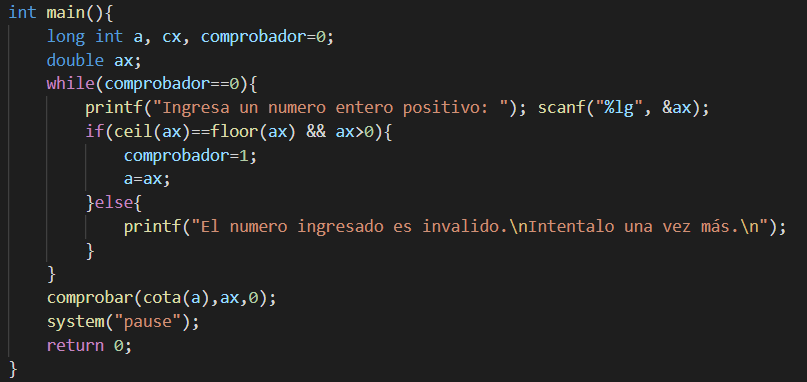
\includegraphics[scale=0.7]{main}
\end{center}
\end{frame}

\begin{frame}
  \frametitle{Explicaci\'on}
  \framesubtitle{Funci\'on principal}
  \begin{itemize}[<+->] % para que parezcan uno a uno
  \item Se crea un comprobador para analizar si el n\'umero introducido es entero positivo.
  \item Se llaman a las funciones que realizan el algoritmo anteriormente descrito.
  \end{itemize}
\end{frame}

\subsection[cota]{cota}

\begin{frame}
  \frametitle{C\'odigo}
  \framesubtitle{Funci\'on de acotaci\'on}
  \begin{center}
 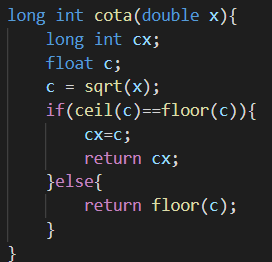
\includegraphics[scale=1]{cota}
\end{center}
\end{frame}

\begin{frame}
  \frametitle{Explicaci\'on}
  \framesubtitle{Funci\'on de acotaci\'on}
  \begin{itemize}[<+->] % para que parezcan uno a uno
  \item Se calcula la ra\'{i}z cuadrada del n\'umero introducido por el usuario.
  \item Si no es entera, se devuelve el entero positivo m\'as cercano al valor de la ra\'{i}z.
  \end{itemize}
\end{frame}

\subsection[comprobar]{comprobar}

\begin{frame}
  \frametitle{C\'odigo}
  \framesubtitle{Funci\'on de comprobaci\'on}
  \begin{center}
 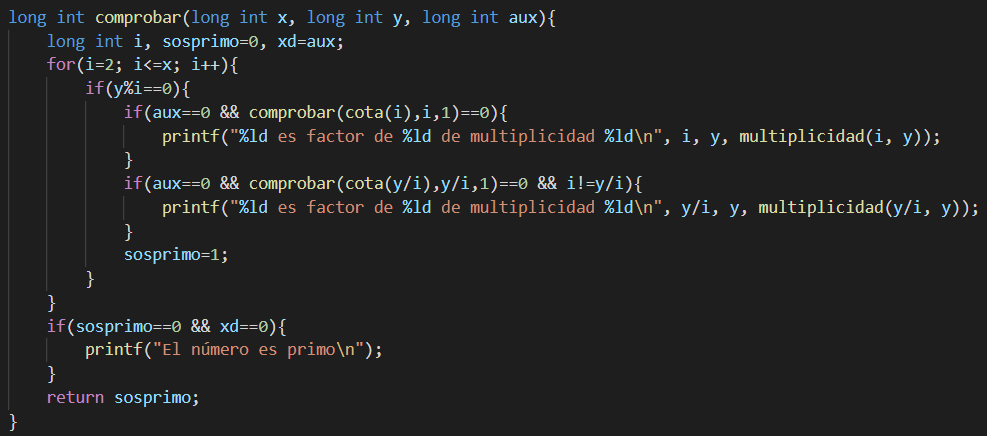
\includegraphics[scale=0.5]{comprobar}
\end{center}
\end{frame}

\begin{frame}
  \frametitle{Explicaci\'on}
  \framesubtitle{Funci\'on de comprobaci\'on}
  \begin{itemize}[<+->] % para que parezcan uno a uno
  \item Se comprueban, uno a uno, los valores desde 2 hasta $\sqrt{n}$.
  \item Se calcula y comprueba $n$ entre el n\'umero comprobado.
  \item Se implementan varias variables auxiliares para evitar imprimir los valores resultado de las comprobaciones paralelas.
  \item Se determina si el n\'umero introducido por el usuario es primo o no, y sus factores.
  \end{itemize}
\end{frame}

\subsection[multiplicidad]{multiplicidad}

\begin{frame}
  \frametitle{C\'odigo}
  \framesubtitle{Funci\'on de calculo de la multiplicidad}
  \begin{center}
 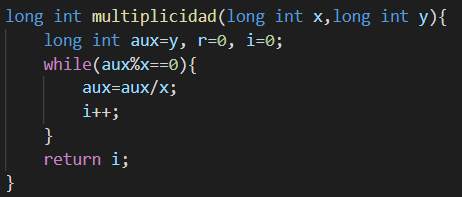
\includegraphics[scale=1]{multiplicidad}
\end{center}
\end{frame}

\begin{frame}
  \frametitle{Explicaci\'on}
  \framesubtitle{Funci\'on de calculo de la multiplicidad}
  \begin{itemize}[<+->] % para que parezcan uno a uno
  \item Con los factores obtenidos en la funci\'on anterior, se calcular mediante un contador la multiplicidad de cada uno.
  \end{itemize}
\end{frame}

\section*{Resumen}

\begin{frame}
  \frametitle{Resumen}

  \begin{itemize}
  \item Se pueden reducir las comprobaciones a s\'olo n\'umeros menores que $\sqrt{n}$.
  \item Como son n\'umero mucho m\'as chicos que $n$, incluso las recursiones para calcular todos los factores son menos demandantes.
  \end{itemize}
  
\end{frame}


\end{document}

